\documentclass[12pt, a4paper]{article}
\usepackage[francais]{babel}
\usepackage{pgfplots}
\usepackage{caption}
\usepackage{graphicx}
\usepackage[T1]{fontenc}
\usepackage{listings}
\usepackage{geometry}
\usepackage{minted}
\usepackage{array,multirow,makecell}
\usepackage[colorlinks=true,linkcolor=black,anchorcolor=black,citecolor=black,filecolor=black,menucolor=black,runcolor=black,urlcolor=black]{hyperref}
\setcellgapes{1pt}
\makegapedcells
\usepackage{fancyhdr}
\pagestyle{fancy}
\lhead{}
\rhead{}
\chead{}
\rfoot{\thepage}
\lfoot{}
\cfoot{}

\renewcommand{\headrulewidth}{0.4pt}
\renewcommand{\listingscaption}{Code}
\renewcommand{\listoflistingscaption}{Table des codes}
% \usepackage{mathpazo} --> Police à utiliser lors de rapports plus sérieux

\begin{document}
\begin{titlepage}
	\newcommand{\HRule}{\rule{\linewidth}{0.5mm}} 
	\center 
	\textsc{\LARGE iut de colmar}\\[6.5cm] 
	\textsc{\Large R303}\\[0.5cm] 
	\textsc{\large Année 2022-23}\\[0.5cm]
	\HRule\\[0.75cm]
	{\huge\bfseries Services réseaux avancés}\\[0.4cm]
	\HRule\\[1.5cm]
	\textsc{\large martin baumgaertner}\\[6.5cm] 

	\vfill\vfill\vfill
	{\large\today} 
	\vfill
\end{titlepage}
\newpage
\tableofcontents
\listoffigures
\newpage
\section{CM 1 - 6 septembre 2022}
\subsection{Rappels}
TCP : permet d'avoir une communication fiable de bout en bout, on a une session 
qui permet de faire du recouvrement, s'il y a un paquet perdu on le retransmet, pour ça on 
utilise un numéro de séquence, et on a un mécanisme d'aquittement qui nous dit quel
octet est arrivé et quel octet est perdu. \\

UDP : est utilisé lorsque l'accusé de réception des données n'a aucune signification, 
est un bon protocole pour les données circulant dans une seule direction,
est simple et adapté aux communications basées sur des requêtes,
n'est pas orienté connexion,
ne fournit pas de mécanisme de contrôle de congestion.\\

\begin{figure}[H]
    \centering
    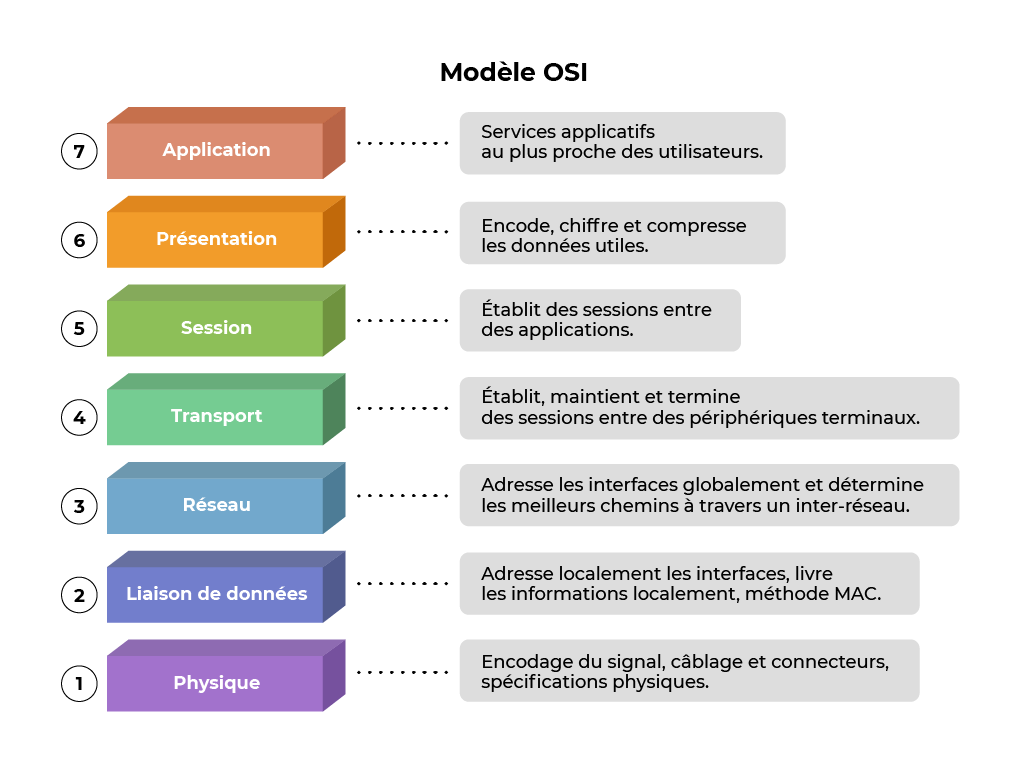
\includegraphics[width=0.9\textwidth]{../img/osi.png}
    \caption{Le modèle OSI}
    \label{fig:osi}
\end{figure}
\newpage
\subsection{Les DNS}
Le Domain Name System (DNS) est une base de données distribuée organisée de manière
hiérarchique, un protocole applicatif qui permet à un hôte de l'intérrroger. Le
port utilisé par défaut pour DNS est le port 53. L'objectif de ce sytème est
d'identifier les hôtes grâce à un nom. \\
Le système DNS est souvent utilisé en amont des protocoles applicatifs comme 
HTTP ou les mails.\\

\begin{figure}[H]
\centering
\begin{tikzpicture}
    \begin{axis}[	grid= major ,
            width=0.7\textwidth ,
            xlabel = {Année} ,
            ylabel = {Nombre (en milliard)} ,
            xmin = 1991, xmax = 2022,
            ymin = 0, ymax = 7 000 000 000,
            legend entries={Nombre site web, Nombre d'internautes},
            legend style={at={(0,1)},anchor=north west}]
        \addplot coordinates {(1991,1) (2001,29 000 000) (2011,346 000 000) (2022,2 000 000 000) }; % Tracé point à point
        \addplot coordinates {(2000,414 000 000) (2005,1 000 000 000) (2011,2 000 000 000) (2022,5 000 000 000) }; % Tracé point à point
       
    \end{axis}
\end{tikzpicture}
\caption{Nombre de site web et d'internautes en fonction des années}
\end{figure}
    
    \subsubsection{Fonctionnement du DNS}
    Le DNS gère la distribution du trafic : distribue les informations
    reçus sur le site voulu sur les 2 adresses IP du site.
    Un serveur racine du DNS est un serveur DNS qui répond aux requêtes qui concernent les noms de
    domaines du premier niveau et qui les redirige vers le serveur DNS de premier niveau concerné.
    Bien qu'il puisse exister d'autres hiérarchies de systèmes de noms de domaine (DNS) avec des serveurs
    racine alternantifs, "serveur racine du DNS" est généralement utilisé pour 
    désigner l'un des serveurs racine du DNS d'internet gégé sous l'autorité de L'ICANN.
\newpage 
\subsection{Créer des raccourcis (alias)}
Un alias est un raccourcis dans l'URL d'un site web, on peut donc passer de \\www.iutc078.uha.fr.iut.colmar.fr
à www.iutc078.uha.fr. La version complète se nomme version canonique.

\subsubsection{Petit exercice pour vendredi prochain}
Comment on gère un cache\\

Un cache est un ensemble de réponses de requêtes faites précédemment 
sur une page web et qui ont été préalablement recueillies. Une clé 
d’identification est rattachée à chacune de ces réponses, chaque clé est 
différente. Dans le cas où une requête correspond à une clé d’identification 
déjà identifiée, alors il fourni une réponse instantanée sans refaire appel 
au serveur d’origine. Il facilite donc votre navigation et augmente sa rapidité.
Le gestionnaire de cache prend en charge les mises à jour ainsi que la 
suppression des réponses dans le stockage cache. Il est mis à la disposition 
des utilisateurs dans l’action lancée, avant de répandre la demande vers le 
serveur.\\

Considérons une liste de trois éléments (x1, x2, x3) montrer que le traitement de la 
séquence par un algorithme optimal hors-ligne se fait avec un coup de 8.

\newpage

\section{CM 2 - 9 septembre 2022}
    \subsection{Les Mails}
    \begin{itemize}
        \item  MUA : Mail User Agent, c'est le logiciel qui permet à l'utilisateur de consulter ses mails.
        \item  MTA : Mail Transfer Agent, c'est le logiciel qui permet d'envoyer des mails.
        \item POP : Post Office Protocol, c'est un protocole qui permet de récupérer les mails sur un serveur.
        \item IMAP : Internet Message Access Protocol, c'est un protocole qui permet de récupérer les mails sur un serveur.
        \item MDA : Mail Delivery Agent, c'est un agent de distribution de mail.
    \end{itemize}

    \subsubsection{Contenu d'un mail}
    Dans l'en-tête du mail, on retrouve le Return Push, la liste des serveurs 
    SMTP. Ensuite, il y a un une partie blanche en ASCII puis les données.
    
    \subsubsection{Pertes des données}
    Nous avons aussi des pertes dans un mail. \\
    Les formats sans pertes de données pour un son, est le FLAC. Et pour les
    images c'est le PNG. Mais sur le texte il n'y a aucun algorithme de perte
    de données. \\
    
\newpage
\section{TD 1 - 9 septembre 2022}
    \subsection{Exercice 1}
    \begin{figure}[H]
        \centering
        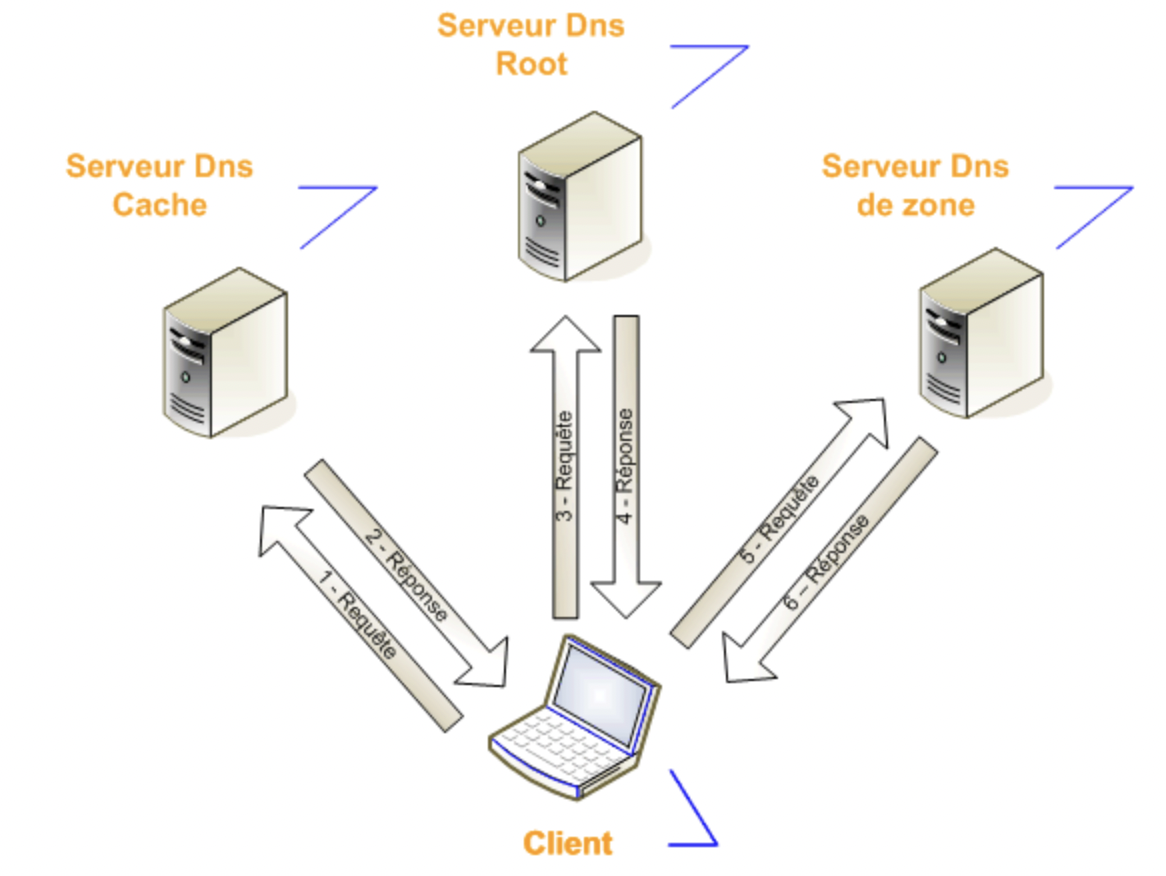
\includegraphics[width=0.6\textwidth]{../img/iteratif.png}
        \caption{La recherche itérative}
        \label{fig:iteratif}
    \end{figure}
    \begin{figure}[H]
        \centering
        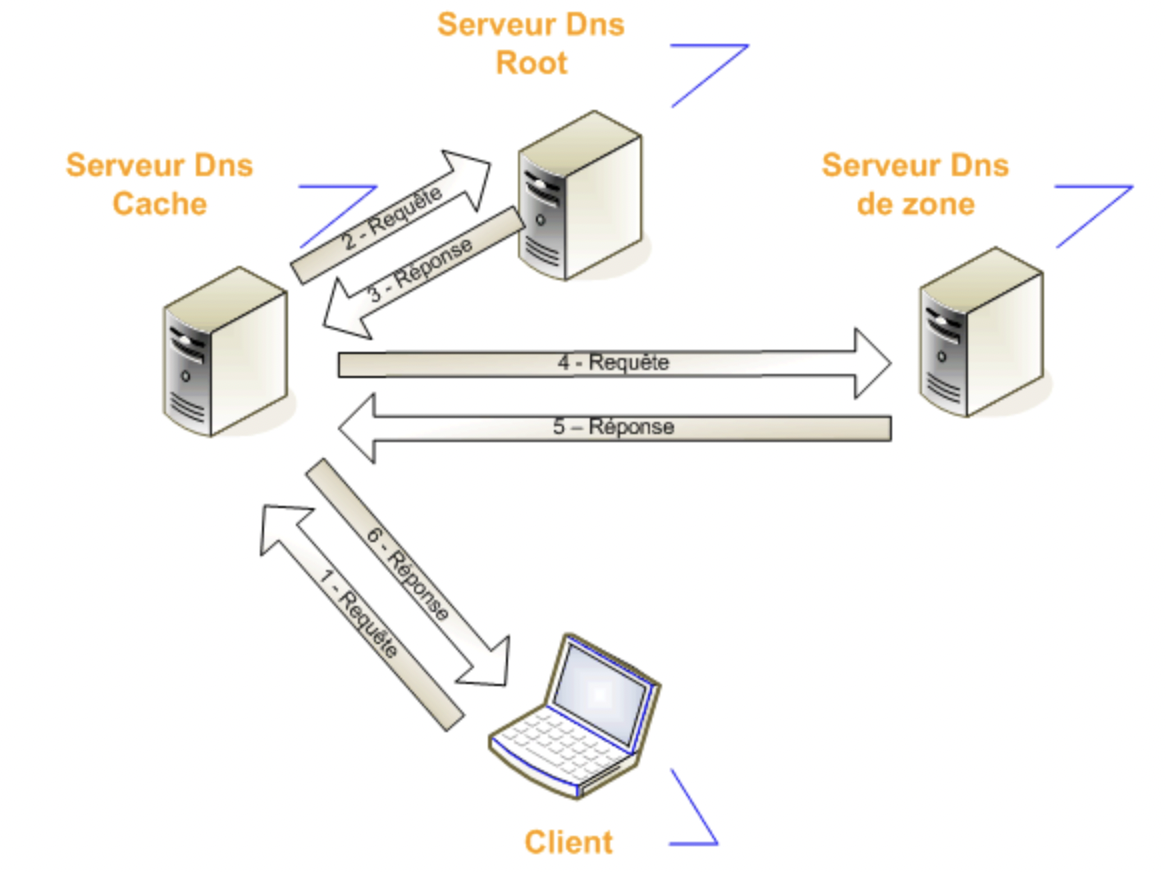
\includegraphics[width=0.6\textwidth]{../img/recursif.png}
        \caption{La recherche récursive}
        \label{fig:recursif}
    \end{figure}
\newpage
Dans la version itérative : www.uha.fr/index.html on fait dans l'ordre la 
recherche de ces éléments : (on va venir demander au résolveur ces informations
dans l'ordre)
\begin{itemize}
    \item 1. \texttt{www} 
    \item 2. \texttt{uha} 
    \item 3. \texttt{fr} 
    \item 4. \texttt{index.html} : ressource
\end{itemize}
    \subsubsection{Algorithme itératif (str, @R)}

    \begin{listing}[H]
        \caption{Algorithme pour la méthode itérative}
        \label{lst:ite}
        \begin{minted}{py}
    liste <- decoupage(str)
    IP <- @R 
    pour index allant de 0 à longueur-1 :
        IP <- résoudre(liste[longueur-index], IP)
    retrouver IP
        \end{minted}
    \end{listing}

    \subsubsection{Algorithme récursif (str, @R)}

    \begin{listing}[H]
        \caption{Algorithme pour la méthode itérative}
        \label{lst:recu}
        \begin{minted}{py}
    si l(str) = 0
        retourne IP
    sinon
        IP <- str([ln(str)], IP)
        supprime dernier élément(str)
            fonction résursive(str,IP)
        \end{minted}
    \end{listing}

\newpage
\section{TP 1 - 13 septembre 2022}
    \subsection{Environnement}
        \subsubsection{Exercice 1}
        Les adresses IP des deux machines sont dans le même réseau. 
        \begin{itemize}
            \item serveur : 192.168.242.130
            \item client : 192.168.242.129
        \end{itemize}
        Les deux machines arrivent bien à se ping.

    \subsection{Configuration du client}
        \subsubsection{Exerice 2}
        Dans la machine client, j'ai modifié l'adresse présente dans le fichier\\ 
        \textit{/etc/resolv.conf} par l'adresse IP du serveur.
        \subsubsection{Exercice 3}
        "Multi on" signifie de dire au résolveur, le système qui traduit les noms 
        d'hôtes en IP, de renvoyer plusieurs listes si elles sont trouvées dans 
        le fichier host. 

    \subsection{Configuration du serveur}
        \subsubsection{Exercice 4}
        La commande \textit{echo master > etc/hostname} permet de changer le nom
        de domaine en \texttt{master}
        \subsubsection{Exercice 5}
        Pour pouvoir faire en sorte que le serveur ping son propre nom, avec la commande 
        \textit{ping master}, il faut ajouter dans le fichier \textit{/etc/hosts}
    
        la ligne suivante : \texttt{192.168.242.130\footnote{adresse IP du serveur} master}
        \subsubsection{Exercice 6}
        \textit{/etc/bind/conf.d/} est le dossier où se trouve les fichiers de 
        configuration de bind. 

        \newpage
        \subsubsection{Exercice 7}
        Tout fonctionne. J'arrive à ping depuis le client en fonction cette commande
        \textit{ping master.rt.iutcolmar.uha.fr} 
        Au préalable, j'ai écris les commandes suivantes dans les fichiers suivants :

        \begin{listing}[H]
            \caption{Fichier : /etc/bind/named.conf.local}
            \label{lst:named}
            \begin{minted}{bash}
            zone "rt.iutcolmar.uha.fr." {
                type master;
                notify yes;
                file "/etc/bind/db.rt.iutcolmar.uha.fr";
            };
            \end{minted}
        \end{listing}

        \begin{listing}[H]
            \caption{Fichier : /etc/bind/db.rt.iutcolmar.uha.fr}
            \label{lst:bind}
            \begin{minted}{bash}
;
; BIND data file for broadcast rt.iutcolmar.uha.fr
;
$TTL    604800
@       IN      SOA     master.rt.iutcolmar.uha.fr. root.rt.iutcolmar.uha.fr. (
        1               ; Serial
        604800          ; Refresh
        86400           ; Retry
        2419200         ; Expire
        604800 )        ; Negative Cache TTL
;
@       IN      NS      master.rt.iutcolmar.uha.fr.
master  IN      A       192
            \end{minted}
        \end{listing}

        Il faut aussi rajouter dans le fichier \textit{/etc/resolv.conf} de la machine
        client les lignes suivantes :

        \begin{listing}[H]
            \caption{Fichier : /etc/resolv.conf}
            \label{lst:resolv}
            \begin{minted}{bash}
                    search localdomain
                    nameserver 192.168.242.130
            \end{minted}
        \end{listing}

        \subsubsection{Exercice 8}
        Pour rajouter un alias qui pointe vers master.rt.iutcolmar.uha.fr, il faut
        ajouter dans le fichier \textit{/etc/bind/db.rt.iutcolmar.uha.fr} la ligne suivante :\\
        \texttt{dns1 IN CNAME master.rt.iutcolmar.uha.fr.} tout à la fin. 

    

        


\end{document}